%
% Compact Device and Macromodel Specification - The Curtice MESFET 
%
% Copyright (C) 2007 Mike Brinson <mbrin72043@yahoo.co.uk>
% Copyright (C) 2007 Stefan Jahn <stefan@lkcc.org>
%
% Permission is granted to copy, distribute and/or modify this document
% under the terms of the GNU Free Documentation License, Version 1.1
% or any later version published by the Free Software Foundation.
%

\tutsection{Introduction}

The Metal and Semiconductor FET (MESFET) is a Schottky-barrier gate
FET made from gallium arsenide. It is popular for high frequency
applications because of it's high electron mobility. The device was
developed by Walter R. Curtice\footnote{W.R Curtice, 1980, A MESFET
model for use in the design of GaAs integrated circuits, IEEE
Transactions on Microwave Theory and Techniques, MTT-28, pp. 448-456.}
in 1980 at the RCA Laboratory in Princeton, New Jersey. USA.  The
MESFET model presented below is based on a Qucs equation defined
device (EDD) which functions as a Curtice level 1 MESFET model with
interelectrode capacitances. Basic temperature effects are also
included.

\tutsection{Qucs EDD model for the Curtice MESFET}
\begin{figure}
  \centering 
  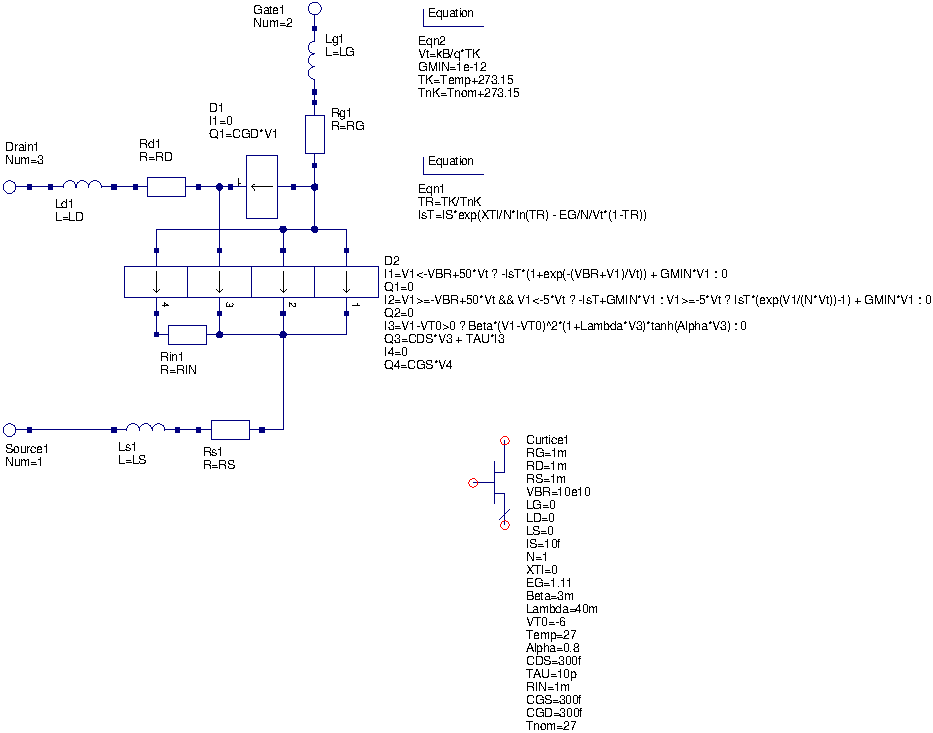
\includegraphics[width=1.0\linewidth]{APPC_fig1}
  \caption{A Qucs EDD model for the Curtice MESFET}
  \label{fig:APPC_fig1}
\end{figure} 

Parameters

\begin{longtable}{rllll}
Name & Symbol & Description & Unit & Default\\
\hline
\endhead
RG & $R_{G}$ & external gate resistance & $\ohm$ & $1\milli$\\
RD & $R_{D}$ & external drain resistance & $\ohm$ & $1\milli$\\
RS & $R_{S}$ & external source resistance & $\ohm$ & $1\milli$\\
VBR & $V_{DR}$ & GS breakdown voltage & $\volt$ & $10^{10}$\\
LG & $L_{G}$ & external gate lead inductance & $\henry$ & $0$\\
LD & $L_{D}$ & external drain lead inductance & $\henry$ & $0$\\
LS & $L_{S}$ & external source lead inductance & $\henry$ & $0$\\
Is & $I_{S}$ & diode saturation current & $\ampere$ & $10\femto$\\
N & $N$ & diode emission coefficient & $$ & $1$\\
XTI & $X_{TI}$ & diode saturation current temperature coefficient & $$ & $0$\\
EG & $E_{G}$ & diode energy gap & eV & $1.11$\\
TAU & $\tau$ & internal time delay from drain to source & $\second$ & $10\pico$\\
RIN & $R_{IN}$ & series resistance to CGS & $\ohm$ & $1\milli$\\
CGS & $C_{GS}$ & interelectrode gate-source bias-independent & $\farad$ & $300\femto$\\
 &  & capacitance &  & \\
CGD & $C_{GD}$ & interelectrode gate-drain bias-independent & $\farad$ & $300\femto$\\
 &  & capacitance &  & \\
CDS & $C_{DS}$ & interelectrode drain-source bias-independent & $\farad$ & $300\femto$\\
 &  & capacitance &  & \\
Tnom & $T_{NOM}$ & device parameter measurement temperature & $\celsius$ & $27$\\
Temp & $T$ & device temperature & $\celsius$ & $27$\\
Alpha & $\alpha$ & coefficient of Vds in tanh function for & $1/\volt$ & $0.8$\\
 &  & quadratic model &  & \\
Beta & $\beta$ & transconductance parameter & $\ampere/\volt^2$ & $3\milli$\\
Lambda & $\lambda$ & channel length modulation parameter for & $1/\volt$ & $40\milli$\\
 &  & quadratic model &  & \\
VTO & $V_{TO}$ & quadratic model gate threshold voltage & $\volt$ & $-6$\\
\end{longtable}

\tutsection{The MESFET equations}

\begin{itemize}
 \item DC characteristics
\begin{enumerate}
 \item for $\left( V_{GS}<-V_{BR}+50 \cdot V_T\right)$
 \begin{equation}
I_{GS} = -I_S\left(T\right)\cdot\left(1+\exp\left( -\dfrac{V_{BR}+V_{GS}}{V_T}\right)\right)  + G_{MIN} \cdot V_{GS}
\end{equation} 
 \item for $\left( V_{GS}>=-V_{BR}+50 \cdot V_T\right)$ and $\left( V_{GS}<-5 \cdot V_T\right)$
 \begin{equation}
 I_{GS}= -I_S\left(T\right)+G_{MIN} \cdot V_{GS}
       \end{equation} 
 \item for $\left( V_{GS}>=-5 \cdot V_T \right)$
 \begin{equation}
  I_{GS}=I_S\left(T\right)\cdot\left( \exp\left(\dfrac{V_{GS}}{N \cdot V_T}\right) - 1\right) + G_{MIN} \cdot V_{GS}
       \end{equation} 
 \item for $\left(V_{GS}-V_{TO}\right)>0$
 \begin{equation}
        I_{DS}=\beta\cdot\left( V_{GS}-V_{TO}\right)^{2}\cdot\left( 1+\lambda \cdot V_{DS}\right)\cdot \tanh\left( \alpha \cdot V_{DS}\right)
       \end{equation} 

       
\end{enumerate}

Where
\begin{equation}
 I_S\left(T\right)=I_S \cdot \exp\left( \dfrac{X_{TI}}{N}\cdot\ln(TR)-\left(  E_G/N/V_T\right)\cdot\left(1-TR\right)\right)  
\end{equation} 
\begin{equation}
 Tr=\dfrac{TK}{TnK}\hspace{3mm} \textrm{ and }  \hspace{3mm} TK=T+273.15, \hspace{3mm} TnK=T_{NOM}+273.15
\end{equation} 

\item MESFET charge equations

\begin{enumerate}
 \item \begin{equation}
        Q_{GS} = C_{GS} \cdot V_{GS}
       \end{equation} 
 \item \begin{equation}
        Q_{GD} = C_{GD} \cdot V_{GD}
       \end{equation} 
 \item \begin{equation}
        Q_{DS} = C_{DS} \cdot V_{DS} + \tau \cdot I_{DS}
       \end{equation} 
\end{enumerate}
\end{itemize}

\newpage
\tutsection{Test circuits and simulation results}

\begin{figure} [h]
  \centering 
  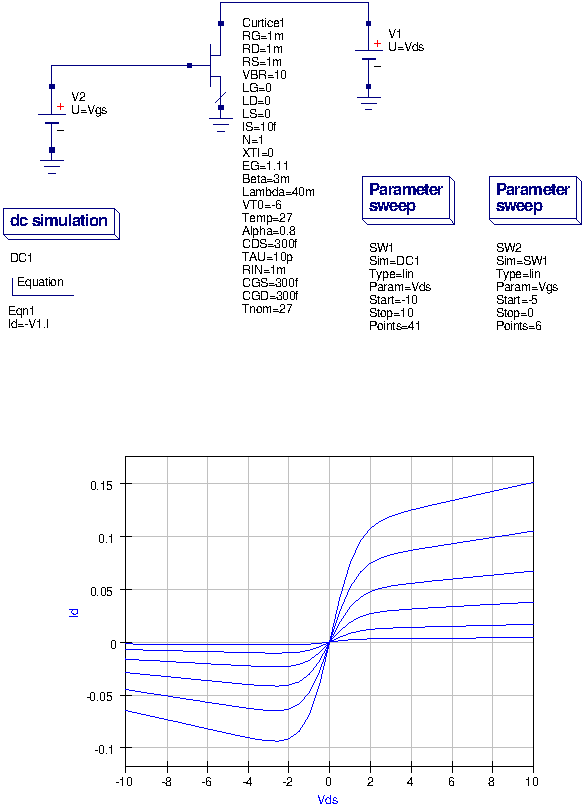
\includegraphics[width=0.7\linewidth]{APPC_fig2}
  \caption{DC test circuit and Id-Vds characteristics}
  \label{fig:APPC_fig2}
\end{figure} 

\begin{figure}
  \centering 
  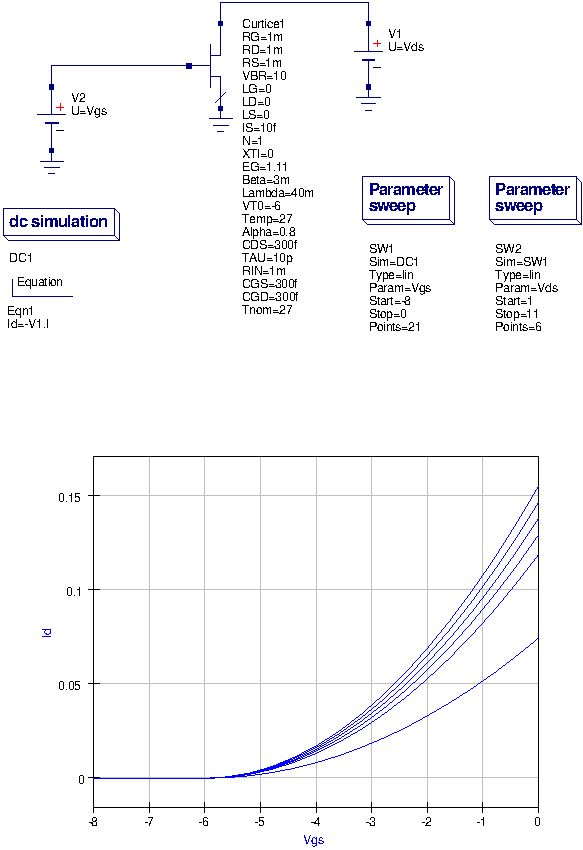
\includegraphics[width=0.9\linewidth]{APPC_fig3}
  \caption{DC test circuit and Id-Vgs characteristics}
  \label{fig:APPC_fig3}
\end{figure} 


\begin{figure}
  \centering 
  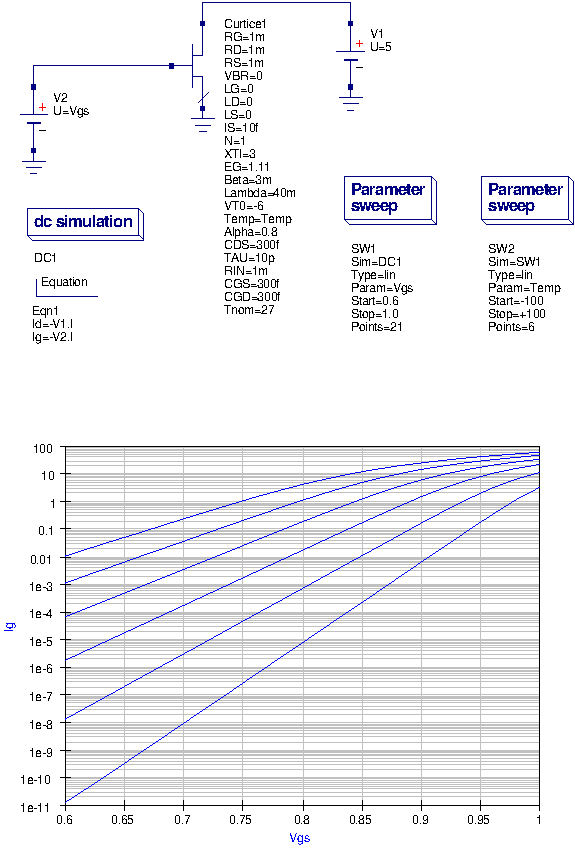
\includegraphics[width=0.85\linewidth]{APPC_fig4}
  \caption{DC test circuit and Ig-Vgs characteristics}
  \label{fig:APPC_fig4}
\end{figure} 

\begin{figure}
  \centering 
  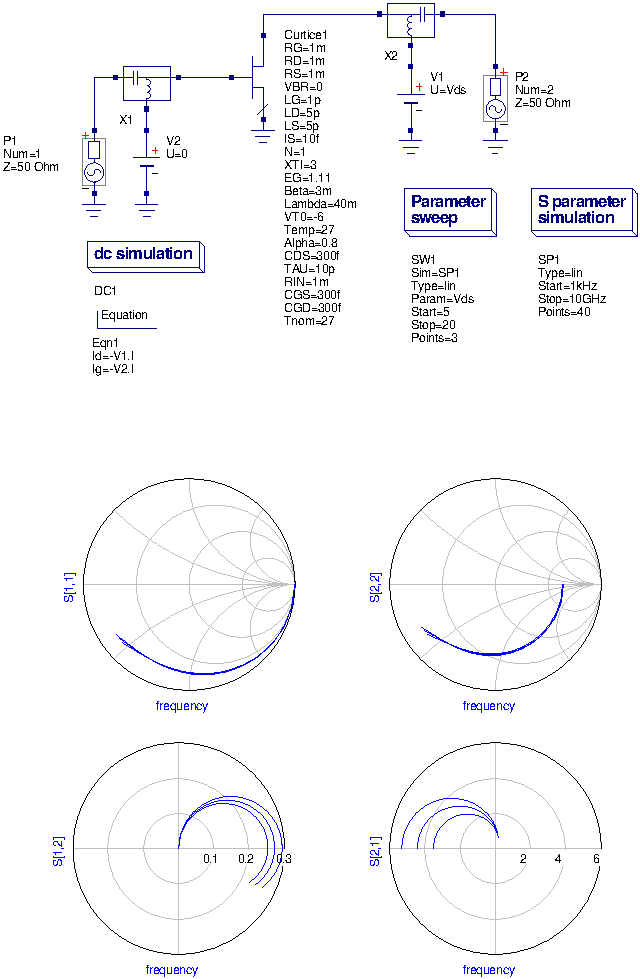
\includegraphics[width=0.85\linewidth]{APPC_fig5}
  \caption{S parameter test circuit and characteristics}
  \label{fig:APPC_fig5}
\end{figure} 



